% Chapter 7

\chapter{Mechanized behavioural semantics} 
\label{chap:behaviour} 

\epigraph{\textit{“The greater danger for most of us lies not in setting our aim too high and falling short; but in setting our aim too low, and achieving our mark."}}{Michelangelo}



\minitoc


\lhead{Chapter 7. \emph{Mechanized behavioural semantics}} % This is for the header on each page - perhaps a shortened title

%----------------------------------------------------------------------------------------

	This chapter discusses the mechanization, in the Coq proof assistant, of a behavioural 
semantics based on the execution trace of synchronized labelled transition systems. Further, we show
how it can be used in the context of \ac{GCM} applications.

	Section \ref{sec:groundwork} briefly presents the encoding of infinite data structures in Coq.	
	Then, section \ref{sec:pLTS} presents the mechanization of \ac{LTS}s and
their traces. We show how we can synchronize several \ac{LTS}s in Section \ref{sec:pnet}.
Then, we exemplify its use in the context of \ac{GCM} applications in Section \ref{sec:gcmpnets}.
For last, Section \ref{sec:behaviourdiscussion} discusses the final remarks about this
mechanization.



\section{Groundwork: Infinite data structures}
\label{sec:groundwork}

	In this section we briefly discuss the concepts involved in the definition of infinite data structures such as lazy lists.	
	For a more detailed coverage of these topics the interested
	reader is pointed to \cite[chap. 13]{opac-b1101046}.


	As discussed in Section \ref{sec:coq}, values from an inductive type are obtained by repeated application of
	its constructors. Further, the type's induction principle constrains this sequence of constructor application
	to be finite. On the other hand, while values from \textit{co-inductive} types are also obtained via repeated 
	application of its constructors, there is no such infinity restriction.

	One of the most basic co-inductive types is the one encoding \textit{lazy lists}. Listing \ref{lst:llist}
	encodes its datatype.
	
			\lstinputlisting[language=Coq, stepnumber=1, 
	                      caption={\textsf{LList} datatype}, 
	                      %firstnumber=19,
	                      label=lst:llist]{listings/chapter6/llist.tex}	
	
	\noindent Indeed, its definition follows the definition of an inductive list.	
	Its only difference lies in the use of the \textsf{CoInductive} keyword.
	Yet, there is a fundamental distinction in that this datatype allows to build
	infinite lists.
	
		For instance, one can easily build a list holding the infinity of natural numbers as
	depicted by Listing \ref{lst:nats}.
	
	
				\lstinputlisting[language=Coq, stepnumber=1, 
	                      caption={Lazy list holding all natural numbers}, 
	                      %firstnumber=19,
	                      label=lst:nats]{listings/chapter6/nats.tex}	
	
	\noindent Any attempt to reproduce the above with an inductive list would be rejected by
	Coq. Further, the careful reader may notice the use of the \textsf{CoFixpoint} keyword. Indeed,
	it is used in a similar fashion as the \textsf{Fixpoint} keyword, yet, it does not impose
	restrictions forbidding the construction of infinite structures, and thus is very handy when dealing
	with the infinity.



\section{Labelled transition systems, and traces}
\label{sec:pLTS}

\subsection{Encoding labelled transitions systems}
\label{sub:lts}
	
	Let us start by the basic constituent of an \ac{LTS}: a state. Listing \ref{lst:ltsstate} depicts
	its mechanization.	
	
	\lstinputlisting[language=Coq, stepnumber=1, 
	                      caption={\textsf{lts\_state} datatype}, 
	                      %firstnumber=19,
	                      label=lst:ltsstate]{listings/chapter6/state.tex}	
	
	
	\noindent A \textsf{lts\_state} is identified by a natural number, and holds an internal memory that is a
	simple mapping between strings to naturals. For the sake of simplicity we directly use strings to denote variables,
	and constrain ourselves to natural number values.
	
	Next, let us now see the \textsf{action} datatype. Listing \ref{lst:action} illustrates its definition.
	
		\lstinputlisting[language=Coq, stepnumber=1, 
	                      caption={\textsf{action} datatype}, 
	                      %firstnumber=19,
	                      label=lst:action]{listings/chapter6/action.tex}	

	\noindent An \textsf{action} is composed by a \textsf{message}, and a set of \textsf{assignments}.
	As expected, the latter permits to specify the assignment of specific state variables to a \textsf{transition}.
	The former holds the label, its type of communication and a set of parameters. Listing \ref{lst:message}
	depicts its definition.
	
			\lstinputlisting[language=Coq, stepnumber=1, 
	                      caption={\textsf{message} datatype}, 
	                      %firstnumber=19,
	                      label=lst:message]{listings/chapter6/message.tex}	

	\noindent A message can either be \textit{reading} or \textit{emitting} (lines 2-3). Typically, these
	are used to receive and transmit values, respectively. Naturally, the allowed \textsf{parameters} are
	either values --- natural numbers --- or variables (lines 6-7).
	
	
	Finally, we can now see the \textsf{LTS} datatype as depicted by Listing \ref{lst:lts}.	
		
	\lstinputlisting[language=Coq, stepnumber=1, 
	                      caption={\textsf{LTS} datatype}, 
	                      %firstnumber=19,
	                      label=lst:lts]{listings/chapter6/LTS.tex}	


\subsection{LTS traces}
\label{sub:ltstrace}


	Having defined the \textsf{LTS} datatype, we can now define \textsf{traces}. A trace is a sequence of actions 
	resulting from the sequence of \textsf{transitions} taken by the \textsf{LTS}. It can either be finite or
	infinite. A finite trace means that a \textit{sink} state was attained, thus the execution \textit{deadlocks}.
	Listing \ref{lst:ltstrace} defines a \textsf{LTS} trace.	
	
	
		\lstinputlisting[language=Coq, stepnumber=1, 
	                      caption={Trace definition for a \textsf{LTS}}, 
	                      %firstnumber=19,
	                      label=lst:ltstrace]{listings/chapter6/ltstrace.tex}	


	\noindent A \textsf{LTS\_Trace} is defined by a co-inductive predicate since we potentially deal
	with infinite sequences. The expression, \textsf{LTS\_Trace A q l}, means that \textsf{l} is a trace
	in the \textsf{LTS} object \textsf{A}, starting from the state \textsf{q}.   

		The \textsf{LTS\_Trace} predicate is composed by two constructors: \textsf{lts\_empty\_trace} (line 2)
	and \textsf{lts\_cons\_trace} (line 8).  The former simply expresses that, from any state, 
	all \textsf{actions} of the \textsf{LTS} yield no target state (lines 3-5). Indeed, the
	function 
	\textsf{lts\_target\_state : LTS $\rightarrow$ lts\_state $\rightarrow$ message $\rightarrow$ lts\_state}
	is responsible for computing the attained state from \textsf{q} with an \textsf{action} holding the message
	\textsf{m}. Thus, the constructor's conclusion is \textsf{LTS\_Trace A q LNil}, since the trace from \textsf{q}
	is empty.	The latter constructor however, demands the that we reach a state \textsf{q'} (line 11), and
	a trace from \textsf{q'} (line 12), in order to conclude \textsf{LTS\_Trace A q (LCons (Action m asgns) l)} (line 13).
	
		For the sake of clarity, Listing \ref{lst:ltstargetstate} depicts the \textsf{lts\_target\_state} function.	
	
		\lstinputlisting[language=Coq, stepnumber=1, 
	                      caption={\textsf{lts\_target\_state} function definition}, 
	                      %firstnumber=19,
	                      label=lst:ltstargetstate]{listings/chapter6/ltstargetstate.tex}			
	
	
	\noindent The function pattern matches the \textsf{message m} and checks whether its label
	is equal to \textsf{"-"}. If it is the case then it simply returns the current state \textsf{st} (line 19),
	otherwise it proceeds by calling the \textsf{lts\_get\_target\_state} function (line 20).
	The is due to the fact that we consider a \textsf{message} with a \textsf{"-"} label as
	a special case. As we shall see in Section \ref{sec:pnet}, this exception is related with the 
	way we deal with synchronization between \ac{LTS}.
	
	The \textsf{lts\_get\_target\_state} function starts by pattern matching on the \textsf{LTS}
	list of \textsf{transitions} (line 3),  returning no state if its empty (line 4). If it is not the 
	case (line 5), then we check if the \textsf{transition} at the head of the list possesses
	a source state that matches the parameter state \textsf{st}, and if the \textsf{message} contained
	in its \textsf{action} is equal to the parameter \textsf{message m} (line 6). Should that be the case,
	then it simply process the assignments associated with the taken \textsf{action} (line 9), and updates
	the target state memory accordingly (line 10). As expected, this the the purpose of the
	\textsf{process\_assignment : state\_mem $\rightarrow$ assignments $\rightarrow$ state\_mem} function, 
	and \textsf{-$>>$} notation, respectively. Otherwise it recurs on the tail of the list of 
	\textsf{transitions} (line 13).


\section{Synchronization of LTS, and traces}
\label{sec:pnet}


	In the previous Section we saw how to model a single \ac{LTS}. However, it is often the case
	that we want to be able to have several \ac{LTS} communicate with each other.	This is achieved
	by synchronizing their \textsf{actions}.


\subsection{Encoding synchronizations between LTSs}	
\label{sub:synchencode}	
	
	
		First, let us formalize the notion of a synchronization vector. Listing \ref{lst:synchvectors}
	depicts its datatype.	
	
	\lstinputlisting[language=Coq, stepnumber=1, 
                      caption={\textsf{SynchronizationVector} datatype}, 
                      %firstnumber=19,
                      label=lst:synchvectors]{listings/chapter6/synchvectors.tex}		

	\noindent Basically, a synchronization vector is composed by a list of synchronization elements,
	and an output element (line 9). The former indicate the \textsf{actions} that need to be considered among
	the list of \ac{LTS} being synchronized. The latter stands for the resulting global action.  
	Both synchronization and output elements are represented by string values. For the sake of convenience
	we also permit synchronization elements to be defined through the \textsf{WildCard} constructor (line 2).
	Further we define a notation as depicted by Listing \ref{lst:synchvectorsnotation}.
	
	\lstinputlisting[language=Coq, stepnumber=1, 
                      caption={A convenient notation for \textsf{SynchronizationVector}}, 
                      %firstnumber=19,
                      label=lst:synchvectorsnotation]{listings/chapter6/synchvectorsnotation.tex}	
                      	
    \noindent Basically, it permits Coq to directly understand expressions such 
    as the following one: \textsf{$<<$ "x" , "y" , "-" , "z" $>>$ -> "XYZ"} --- from left to right,
    four \textsf{LTS} objects are synchronized on their \textsf{actions} labelled \textsf{"x"}, \textsf{"y"}, any,
    and \textsf{"z"}, respectively, yielding a global \textsf{action} labelled \textsf{"XYZ"}.

	Let us now define a type for a communicating network of \ac{LTS}. We shall call this type \textsf{Net}.
	Its definition is depicted by Listing \ref{lst:net}.	

	\lstinputlisting[language=Coq, stepnumber=1, 
                     caption={\textsf{Net} datatype}, 
                     %firstnumber=19,
                     label=lst:net]{listings/chapter6/net.tex}	

	\noindent It is composed by two constructors: \textsf{mk\_SingletonNet} and \textsf{mk\_Net}.
	The former is used for simple models constituted with a single \ac{LTS}, while the latter
	permits to specify communicating \ac{LTS} by means of synchronization vectors.
	
	For this new structure we need a new notion of state. Listing \ref{lst:netstate} depicts the \textsf{pnet\_state}
	datatype.

	\lstinputlisting[language=Coq, stepnumber=1, 
                     caption={\textsf{net\_state} datatype}, 
                     %firstnumber=19,
                     label=lst:netstate]{listings/chapter6/netstate.tex}	

	\noindent Basically, both its constructors follow the same rationale: they keep track of the 
	involved \textsf{lst\_states}. 
	
	%indexed_membership
	%attainable
	
  \subsection{Net traces}	
\label{sub:nettraces}		
	
	Before proceeding to the definition of traces for	\textsf{Net}s, we need to consider
	how their transitions are performed. For this case, we need to consider the current
	\textsf{net\_state} and the activated synchronization vector. Moreover, each synchronization
	element may permit more than one \textsf{action} to occur. Thus, a function
	computing the target \textsf{net\_state}s must also return the resulting global action.
	Listing \ref{lst:nettargetstates} depicts such a function.
		
	\lstinputlisting[language=Coqfix, stepnumber=1, 
                     caption={\textsf{net\_target\_states} function definition}, 
                     %firstnumber=19,
                     label=lst:nettargetstates]{listings/chapter6/nettargetstates.tex}		
	
	
	\noindent The above function may seem complicated at first sight, and requires 
	a closer look. Basically, it starts by pattern matching on its \textsf{Net} parameter
	\textsf{net\_obj}, \textsf{net\_state} parameter \textsf{q}, and synchronization vector parameter
	\textsf{sv} (line 3). The function is supposed to be used with \textsf{Net} objects and \textsf{net\_state}
	modelling systems with \textsf{LTS} synchronization. Should that not be the case, it simply returns
	an empty list (line 17). The function 
	\textsf{allowed\_actions\_from\_sv\_element : list LTS $\rightarrow$ list lts_state $\rightarrow$ 
	list SyncronizationElement $\rightarrow$ list (list action)} computes the \textsf{actions} that
	may occur at each \textsf{LTS} composing \textsf{llts}, taking into account its current
	\textsf{lts\_state} held at \textsf{sts} and w.r.t the adequate synchronization element
	in \textsf{svs} (line 5). Then, it is necessary to generate all combinations of \textsf{actions}
	that may occur for each \textsf{LTS} (line 6). This is the purpose of the
	\textsf{combineN : list (list action) -> list (list action)} function.  Next, it goes through 
	all generated combinations, and gets for all \textsf{LTS} objects
	the target states along with the message to synchronize (line 11). 
	This is the purpose of the \textsf{get\_target\_lts\_states}
	function. Then,  the functions \textsf{message\_parameter\_to\_emit} and
	\textsf{transmit\_message} take care of the variables passing between
	the synchronized \textsf{LTS} objects. The function 
	\textsf{global\_action\_output} returns the global action
	resulting from the synchronized \textsf{action} labels with their parameters (line 14).
	Finally, the computed global action along with the attained \textsf{pnet\_state} is kept,	
	and the function recurs (line 15). 
	 
		
		Another useful function concerns the computation of the initial state of a \textsf{Net}.
	Listing \ref{lst:initnet} depicts its definition.
	
	\lstinputlisting[language=Coqfix, stepnumber=1, 
                     caption={\textsf{init\_net\_state} function}, 
                     %firstnumber=19,
                     label=lst:initnet]{listings/chapter6/initnet.tex}		
	
	\noindent Basically, the above function proceeds by pattern matching on the \textsf{Net} parameter \textsf{net\_obj} (line 2). 
	If it is a \textsf{Net} with a single \textsf{LTS} object, than it simply returns the adequate \textsf{net\_state}
	constructor with the initial state of the \textsf{LTS} (line 3). Otherwise, it recursively
	gathers the initial state of each \textsf{LTS} objects composing \textsf{net\_obj} into
	the local variable \textsf{lq} (lines 5-9), and returns the adequate \textsf{net\_state}
	constructor with \textsf{lq} (line 10).
	

		Let us now define a predicate indicating whether a state can attain another state. Listing \ref{lst:attainable}
	depicts its formalization.
			
			\lstinputlisting[language=Coq, stepnumber=1, 
                     caption={\textsf{attainable} predicate definition}, 
                     %firstnumber=19,
                     label=lst:attainable]{listings/chapter6/attainable.tex}	
	
		
	\noindent It is composed by two constructors: \textsf{Attain0} and \textsf{AttainN}. Intuitively,
	the former expresses the idea that a \textsf{net\_state} can always attain itself (line 3).
	The latter is slightly more involved. Basically, in order for a \textsf{net\_state} \textsf{qi}
	to attain \textsf{net\_state} \textsf{qf}, there needs to be a \textsf{net\_state} \textsf{qn}
	that belongs to \textsf{qi}'s target states, and \textsf{qf} to be attainable from \textsf{qn}.
	The function \textsf{net\_target\_states} computes \textsf{qi}'s target states (line 7) by using
	one of the specified synchronization vectors (lines 5-6). 
	However, it returns a list of tuples associating a global \textsf{action} with a \textsf{net\_state}.
	Thus, \textsf{qn} needs to belong to the list of elements at the right of each tuple.	
	This is the purpose of the function 
	\textsf{get\_list\_snd : forall X Y : Type, list (X * Y) -> list Y}	(line 8). Then, 
	\textsf{qn} needs to be able to attain \textsf{qf} (line 9). The careful reader may wonder
	about the second predicate parameter that stores the list of already seen \textsf{net\_state}s. 
	There is no point in revisiting already seen \textsf{net\_state}s in order to check 
	attainability. Thus, it is also required that the source \textsf{net\_state} was not already
	previously seen (line 4). Naturally, this is the purpose of the negated predicate
	\textsf{seen : net\_state $\rightarrow$ list net\_state $\rightarrow$ Prop}.
	
			
		As expected, traces for \textsf{Net}s are slightly more involved than traces for \textsc{LTS}. 
	Listing \ref{lst:nettrace} formalizes the notion of trace for the \textsf{Net} datatype.
			

		\lstinputlisting[language=Coq, stepnumber=1, 
                     caption={Trace definition for \textsf{Net}}, 
                     %firstnumber=19,
                     label=lst:nettrace]{listings/chapter6/nettrace.tex}	
	
	\noindent It is composed by three constructors: \textsf{lts\_trace},
	\textsf{net\_empty\_trace} and \textsf{net\_lcons\_trace}.
	The first constructor deals with singleton \textsf{Net}s, and thus relies on
	the previously discussed \textsf{LTS\_Trace} predicate (lines 2-7).		
	The second constructor is meant for empty traces, that is, when there is no
	synchronization vector that can be activated (line 14), 
	and thus the execution is stuck (line 15). Two further requirements are specified.
	First, it is required that the current \textsf{net\_state} \textsf{q} is 
	attainable from the initial state of the \textsf{Net} object \textsf{A} (line 13). Second, 
	the 
	\textsf{indexed\_membership : list lts\_state $\rightarrow$ list LTS $\rightarrow$ Prop}
	predicate simply states that the $i^{th}$ element of the first parameter belongs to the set of \textsf{lts\_states} 
	of the $i^{th}$ element of the second parameter (line 12).
	%These two requirements serve the purpose of constraining 
	The third constructor deals with the most interesting case: there is a successful synchronization
	between the \ac{LTS}s composing the \textsf{Net} object \textsf{A}. As in the second constructor,
	the indexed membership and attainability requirements are also included (lines 20-21). 
	Further, the expression
	\textsf{net\_target\_states A q sync\_vec} (line 23) yields a list of tuples holding the 
	target states along with the associated global \textsf{action} from 
	\textsf{net\_state} \textsf{q}, and by using 
	a synchronization vector \textsf{sync\_vec} belonging to \textsf{list\_sv} (line 22).
	Finally, it is necessary to establish 
	a trace from one of the \textsf{net\_state}s belonging	
	to this list of tuples (line 24), and the associated global action 
	is added to the trace (line 25).	
	
		
		
\subsection{Synchronized Master \& Slave example}	
\label{sub:masterslave}

	
		First, let us define a convenient notation for reasoning over execution traces.
	Listing \ref{lst:sat} depicts such definition.
	
					\lstinputlisting[language=Coq, stepnumber=1, 
	                      caption={Definition of the \textsf{satisfies} predicate}, 
	                      %firstnumber=19,
	                      label=lst:sat]{listings/chapter6/sat.tex}	


	\noindent Basically, it permits to use the convenient and familiar notation \textsf{t $\vDash$ p}, meaning
	"trace \textsf{t} satisfies property \textsf{p}". As expected, we shall use a temporal logic in order to reason 
	about such traces. In particular, we take advantage of the encoding in Coq of \ac{LTL} from
	\cite[sec. 13.9]{opac-b1101046}. For the sake of completeness, we demonstrate here a part of 
	this formalization. For instance, Listing \ref{lst:always} depicts the \textsf{Always} predicate.
	
	%Listing \ref{lst:atomic} depicts the \textsf{Atomic} predicate.

	%\lstinputlisting[language=Coq, stepnumber=1, 
	 %                     caption={Definition of the \textsf{atomic} predicate}, 
	                      %firstnumber=19,
	  %                    label=lst:atomic]{listings/chapter6/atomic.tex}	


	%\noindent This is a rather simple predicate. Basically, a stream satisfies the \textsf{Atomic}
	%predicate provided that its head element satisfies the \textsf{At} predicate given as parameter.

  \lstinputlisting[language=Coq, stepnumber=1, 
	                      caption={Definition of the \textsf{Always} predicate}, 
	                      %firstnumber=19,
	                     label=lst:always]{listings/chapter6/always.tex}	
	
	\noindent Basically, the \textsf{Always} predicate holds if the trace  
	satisfies the predicate \textsf{P} given as parameter (line 3), and the \textsf{Always} predicate
	itself must hold for the tail of the trace (line 4). Naturally, it is implicit that this 
	predicate only holds for infinite traces.

	In Section \ref{sec:fiacre} we discussed the Fiacre specification language by illustrating a 
	Master/Slave example from the online Fiacre tutorial. In the following, we show how to encode
	and reason about such system.
	
	
\subsubsection{The slave process}	
\label{subsub:slave}
	
		Let us start by encoding the slave process. It possesses two states. Listing \ref{lst:slavestates}
		depicts their mechanization.
		
  \lstinputlisting[language=Coq, stepnumber=1, 
	                      caption={Definition of the slave process \textsf{lts\_states}}, 
	                      %firstnumber=19,
	                     label=lst:slavestates]{listings/chapter6/slavestates.tex}	


	\noindent Further, it features three kinds of \textsf{actions}: parameterless \textsf{ready} and \textsf{order:MakeSandwich},
	and \textsf{order:MakeCoffee} taking one natural number specifying a kind of coffee. These are encoded as depicted by
	Listing \ref{lst:slaveactions}

	 \lstinputlisting[language=Coq, stepnumber=1, 
	                      caption={Definition of the slave process \textsf{actions}}, 
	                      %firstnumber=19,
	                     label=lst:slaveactions]{listings/chapter6/slaveactions.tex}	

	\noindent Moreover, we need to specify its transitions. This is achieved by the function depicted
	by Listing \ref{lst:slavetransitions}.

		 \lstinputlisting[language=Coq, stepnumber=1, 
	                      caption={Definition of the slave process \textsf{transitions}}, 
	                      %firstnumber=19,
	                     label=lst:slavetransitions]{listings/chapter6/slavetransitions.tex}	

	\noindent Finally, we can now define the \textsf{LTS} representing the slave process as
	demonstrated by Listing \ref{lst:slavelts}.
	
			 \lstinputlisting[language=Coq, stepnumber=1, 
	                      caption={Definition of the slave process \textsf{LTS}}, 
	                      %firstnumber=19,
	                     label=lst:slavelts]{listings/chapter6/slavelts.tex}	


\subsubsection{The master process}	
\label{subsub:master}

	The master process follows the same rationale, except that it emits orders whereas the slave
	receives them. Listing \ref{lst:masterstates} depicts its states.
	
			 \lstinputlisting[language=Coq, stepnumber=1, 
	                      caption={Definition of the master process \textsf{lts\_states}}, 
	                      %firstnumber=19,
	                     label=lst:masterstates]{listings/chapter6/masterstates.tex}	

	\noindent Listing \ref{lst:masteractions} depicts its \textsf{actions}.

	\lstinputlisting[language=Coq, stepnumber=1, 
	                      caption={Definition of the master process \textsf{actions}}, 
	                      %firstnumber=19,
	                     label=lst:masteractions]{listings/chapter6/masteractions.tex}	

	\noindent Its transitions are also encoded via a function as demonstrated by 
	Listing \ref{lst:mastertransitions}.
	
		\lstinputlisting[language=Coq, stepnumber=1, 
	                      caption={Definition of the master process \textsf{transitions}}, 
	                      %firstnumber=19,
	                     label=lst:mastertransitions]{listings/chapter6/mastertransitions.tex}		
	
	\noindent And finally Listing \ref{lst:masterlts} depicts the \textsf{LTS} of the master process.
	
	
			\lstinputlisting[language=Coq, stepnumber=1, 
	                      caption={Definition of the master process \textsf{LTS}}, 
	                      %firstnumber=19,
	                     label=lst:masterlts]{listings/chapter6/masterlts.tex}			
	

	
\subsubsection{Synchronization and a first proof}	
\label{subsub:synch}	
	
	
	Having defined the slave and master processes we now need to specify how they synchronize.
	Listing \ref{lst:mssynch}	depicts their synchronization.	
	
				\lstinputlisting[language=Coq, stepnumber=1, 
	                      caption={Definition of the master process \textsf{LTS}}, 
	                      %firstnumber=19,
	                     label=lst:mssynch]{listings/chapter6/mssynch.tex}		
	
	\noindent Indeed, by using the previously defined notation we can easily specify
	the adequate synchronization vectors. Moreover, specifying the \textsf{Net} of the
	overall system is now a rather simple task.	
	It is depicted by Listing \ref{lst:msnet}.

		\lstinputlisting[language=Coq, stepnumber=1, 
	                      caption={Definition of the overall \textsf{Net}}, 
	                      %firstnumber=19,
	                     label=lst:msnet]{listings/chapter6/msnet.tex}		

	\noindent Having defined this parametrized master/coffee \textsf{Net}, we can
	now try to prove properties about it. For instance, we can show that all traces
	of this system are an infinite interleaving between \textsf{ready} and \textsf{order}
	\textsf{actions}. For this, we first need to define a predicate expressing
	this interleaving. Listing \ref{lst:interleaving} depicts such predicate.

			\lstinputlisting[language=Coq, stepnumber=1, 
	                      caption={Definition of the \textsf{interleaving} predicate}, 
	                      %firstnumber=19,
	                     label=lst:interleaving]{listings/chapter6/interleaving.tex}		

	\noindent It is defined in a polymorphic manner for the sake of genericness.
	As we shall see later, the types \textsf{X} and \textsf{Y} will be instantiated to
	\textsf{action} and \textsf{string}, respectively.			
	Moreover, it features two constructors: \textsf{InterleavingOne} and \textsf{InterleavingTwo}.
	Both possess a similar structure, their only difference lies in the order
	by which the \textsf{actions} occur (lines 4 and 9). Further, the reader may wonder about
	the predicate \textsf{R : Y $\rightarrow$ X $\rightarrow$ Prop} declared as parameter.
	This has the purpose of comparing the actual \textsf{actions} occurring in the
	trace --- \textsf{a'} and \textsf{b'} --- with labels passed as parameter --- \textsf{a} and \textsf{b}. 
	For instance, for the purposes of this example the relation that we use is depicted by Listing \ref{lst:rel}.	
	
		\lstinputlisting[language=Coq, stepnumber=1, 
	                      caption={Definition of the \textsf{Rma} relation}, 
	                      %firstnumber=19,
	                     label=lst:rel]{listings/chapter6/rel.tex}		

	\noindent Its understanding should pose no doubt. Basically, it pattern matches
	the parameters \textsf{l} and \textsf{act}, and checks if \textsf{l} matches 
	the label of the \textsf{message} composing \textsf{act}.
	
	Finally, we are in a position to establish our first proof about traces. Theorem
	\ref{th:msproof2} expresses that from all states, all traces of \textsf{MasterSlaveCoffeeNet} instantiated with three --- 0, 1 and 2 ---
	coffee kinds, satisfy an infinite interleaving between \textsf{ready} \textsf{actions} and \textsf{order}
	\textsf{actions}.
	

\begin{theorem} \label{th:msproof2} 
	\lstinputlisting[language=Coq, numbers=none, nolol=true]{listings/chapter6/msproof2.tex}		
		We start by applying the infamous \textsf{cofix} tactic as this is a proof by co-induction. This
		introduces a hypothesis in our context with the same type as the theorem we are trying to prove.
		We cannot directly use this hypothesis as it would violate Coq's guardedness condition.		
		Instead, we consider all \textsf{Net} trace constructors: \textsf{lts\_trace},
		\textsf{net\_empty\_trace} and \textsf{net\_lcons\_trace}.
		
		For the first case, \textsf{lts\_trace}, the proof is easily discharged as \textsf{MasterSlaveCoffeeNet}
		is a \textsf{Net} value obtained via the \textsf{mk\_Net} constructor, and not with 
		\textsf{NetSingleton\_State}. Thus, we have contradiction in our context.
				
		The second case concerns the \textsf{net\_empty\_trace} constructor. This requires to establish that
		an empty trace, \textsf{LNil}, satisfies the aforementioned infinite interleaving property. Clearly, this is not the
		case, since the trace is empty. Thus, establishing this proof requires to demonstrate a contradiction in our context.
		Since we are universally quantifying over \textsf{q}, we need to consider all possible \textsf{net\_states}. This yields
		four subgoals. For the first subgoal, we consider \textsf{Net_State [slv0; mst0]}	as the source \textsf{net\_state}.
		One of  \textsf{net\_empty\_trace}'s premisses is that \textsf{net\_target\_states} yields no target \textsf{net\_state} for all
		synchronization vectors. This is clearly false, as the can show that \textsf{$<<$ "ready", "ready" $>>$ -> "ready"}
		does indeed permit to attain  \textsf{Net_State [slv1; mst1]}. And thus this subgoal is discharged. For the
		second and third subgoals we have \textsf{Net_State [slv0; mst1]} and \textsf{Net_State [slv1; mst0]}  
		as source \textsf{net\_state}, respectively. Both are supposed to be \textsf{attainable} from \textsf{MasterSlaveCoffeeNet}'s initial
		\textsf{net\_state}. Indeed, this is clearly not the case and we can demonstrate a contradiction.
		The fourth and last subgoal possesses  \textsf{Net_State [slv1; mst1]} as source \textsf{net\_state}, and discharging it follows the rationale
		of the first subgoal except that we use \textsf{$<<$ "order:MakeSandwich", "MakeSandwich" $>>$ -> "order:Sandwich"}
		or \textsf{$<<$ "order:MakeCoffee", "MakeCoffee" $>>$ -> "order:Coffee"} to demonstrate the contradiction.
						
		For last, the third case regards the \textsf{net\_lcons\_trace} constructor. As seen for previous case,
		we need to consider all possible \textsf{net\_states}, thus four subgoals. the third and fourth subgoal
		possess \textsf{Net_State [slv0; mst1]} and \textsf{Net_State [slv1; mst0]}  
		as source \textsf{net\_state}, respectively. By the same reasoning as discussed above, we can demonstrate a contradiction
		in our context. The first subgoal has \textsf{Net_State [slv0; mst0]} as the source \textsf{net\_state}.
		From the three specified synchronization vectors, only 	\textsf{$<<$ "ready", "ready" $>>$ -> "ready"}
		permits the trace to progress: \textsf{Net_State [slv1; mst1]} is reached as target \textsf{net\_state},
		and the global \textsf{action} \textsf{(Action (Message "ready" Emit []) [])} is emitted. We can now apply
		the \textsf{Always\_LCons} constructor, yielding two subgoals. For the first subgoal we need to demonstrate
		that the \textsf{interleaving} predicate holds. For this we make the trace further progress by induction on the
		\textsf{Net\_Trace} predicate in our context, yielding the respective three subgoals. The two first subgoals
		are easily discharged by contradiction in the same manner we discussed above. for the third subgoal
		we need to consider the two synchronization vectors that can be activated: 
		\textsf{$<<$ "order:MakeSandwich", "MakeSandwich" $>>$ -> "order:Sandwich"} and
		\textsf{$<<$ "order:MakeCoffee", "MakeCoffee" $>>$ -> "order:Coffee"}. Since there are three kinds of
		coffee, we need to consider four \textsf{actions}. In all cases we apply the \textsf{InterleavingOne} constructor
		with the adequate \textsf{actions} as parameters, and discharge it by reflexivity. The second subgoal
		for the  \textsf{Always\_LCons} constructor requires to prove the same goal for the tail of the
		trace. For this, we simply use the co-induction hypothesis with \textsf{q} instantiated to
		\textsf{Net_State [slv1; mst1]}. This concludes the first subgoal of the \textsf{net\_lcons\_trace} 
		constructor case. The second and third subgoal were already discussed above, and the fourth is
		discharged analogously. The main difference lies in the fact that  \textsf{Net_State [slv1; mst1]}  
		is the source \textsf{net\_state}, thus the constructor \textsf{InterleavingTwo} is used instead,		
		and a similar reasoning is applied w.r.t. the activated synchronization
		vectors. \qed
\end{theorem}


	The above theorem gives an example on how we can use a proof assistant like Coq to formally reason about
	synchronized transitions systems. Indeed, this is usually achieved by means of automatic techniques such
	as model-checking. Yet, it should be noted that in system like Coq we need not to constrain ourselves
	with finite instances, and can directly reason about parametrized systems. 
	For instance, Listing \ref{lst:msproofn} enunciates the same interleaving property for a parametrized
	\textsf{MasterSlaveCoffeepNet}.

			\lstinputlisting[language=Coq, stepnumber=1, 
	                      caption={Definition of the \textsf{Rma} relation}, 
	                      %firstnumber=19,
	                     label=lst:msproofn]{listings/chapter6/msproofn.tex}		

	Proving the above theorem requires more care as we no longer deal with a closed term.
	In particular, we cannot explicitly enumerate all the \textsf{actions} as they depend on 
	the parameter \textsf{n}.	We perform induction on \textsf{n} and show that
	the set of target states and message labels from the emitted \textsf{actions} never depend on it. 
	In practice, this proof\footnote{At the time of writing, there are still admitted lemmas in the development of this proof. 
	Yet, we feel sufficiently confident on their veracity.}
	follows the same structure as seen for Theorem \ref{th:msproof2} but 	uses auxiliary lemmas 
	dealing with the non-interference of \textsf{n} with the interleaving behaviour.
	
		
		
%%%
\section{Towards GCM behavioural models}
\label{sec:gcmpnets}


	 As seen in Section \ref{sec:pnets}, and further discussed by example throughout Chapter \ref{chap:hyper},
   \ac{GCM} components are internally composed by a set of processes --- \ac{FIFO} \textit{queue}, \textit{body}, 
   etc. These can be modelled with our \textsf{LTS} datatype.
   
   
	For the sake of clarity, Figure \ref{fig:gcmqueue2} depicts a queue, bounded at two requests, and accepting
	requests for method \textsf{m$_1$}.
	
	\begin{figure}[H]
		 \centering
		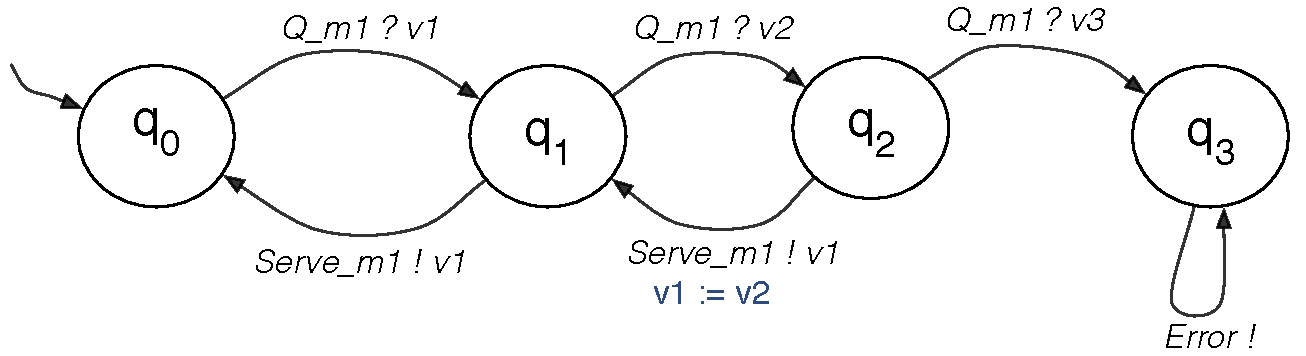
\includegraphics[scale=0.6]{figures/chapter6/gcmqueue2.pdf}
		\caption{LTS of a queue, bounded by two requests}
		\label{fig:gcmqueue2}		
	\end{figure}		
	
	\noindent Its understanding should pose no doubt. \textsf{Action} \textsf{messages} are written
	in \textit{light oblique black} and \textsf{assignments} in blue. Basically, by assigning \textsf{v2} to
	\textsf{v1} after emitting \textsf{Server\_m1 ! v1} it is guaranteed that requests are treated following
	a \ac{FIFO} policy.
		
	
		The mechanization of the above queue is easily achieved using our \textsf{LTS} datatype. First,
		let us see its \textsf{lts\_states} as depicted by Listing \ref{lst:gcmqueue2states}.
		
				
	   	\lstinputlisting[language=Coq, stepnumber=1, 
	                     caption={Encoding of the \textsf{lts\_states} for the queue process}, 
	                     %firstnumber=19,
	                    label=lst:gcmqueue2states]{listings/chapter6/gcmqueue2states.tex}		
	   
   	\noindent Next, Listing \ref{lst:gcmqueue2transitions} illustrates its \textsf{transitions}.
   	
   	 	\lstinputlisting[language=Coq, stepnumber=1, 
	                     caption={Encoding of the \textsf{transitions} for the queue process}, 
	                     %firstnumber=19,
	                    label=lst:gcmqueue2transitions]{listings/chapter6/gcmqueue2transitions.tex}	
 	
 	
	\noindent  Since we use local variables we need to specify them in the initial state as
	shown by Listing \ref{lst:gcmqueue2init}.	
	 	
 	   	 	\lstinputlisting[language=Coq, stepnumber=1, 
	                     caption={Encoding of the initial \textsf{lts\_state} for the queue process}, 
	                     %firstnumber=19,
	                    label=lst:gcmqueue2init]{listings/chapter6/gcmqueue2init.tex}	


	\noindent The last remaining piece is a simple list holding the \textsf{actions}. We omit it
	since they are already represented by the \textsf{transitions} depicted in Listing \ref{lst:gcmqueue2transitions}.
	Finally, we can compose the \textsf{LTS} modelling the queue process. Listing \ref{lst:gcmqueue2}
	illustrates its definition.
	
	\lstinputlisting[language=Coq, stepnumber=1, 
	                       caption={Encoding of the queue process}, 
	                       %firstnumber=19,
	                       label=lst:gcmqueue2]{listings/chapter6/queue2.tex}	


	\noindent A \ac{GCM} component is also composed by a \textit{body} process. Basically, this process
	ensures that \ac{GCM} components are mono-threaded. For instance, a body process handling
	requests for a method \textsf{m$_1$} is depicted by Figure \ref{fig:gcmbody}.


	\begin{figure}[H]
		 \centering
		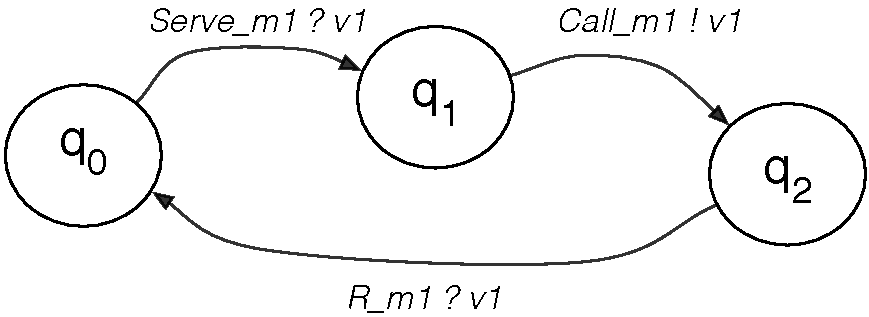
\includegraphics[scale=0.6]{figures/chapter6/gcmbody.pdf}
		\caption{LTS of a body process handling one method}
		\label{fig:gcmbody}		
	\end{figure}		


	\noindent From the above \ac{LTS} we can see that no second process can be \textit{served} without the
	previous one having returned.
	
		The mechanization of the body process follows the same rationale as seen for the queue process.
	Listing \ref{lst:gcmbodytransitions} depicts its transitions.

		\lstinputlisting[language=Coq, stepnumber=1, 
	                       caption={Encoding of the body \textsf{transitions}}, 
	                       %firstnumber=19,
	                       label=lst:gcmbodytransitions]{listings/chapter6/gcmbodytransitions.tex}	
	

	\noindent Further, Listing \ref{lst:gcmbodydef} illustrates the remaining definition of the body process. 

			\lstinputlisting[language=Coq, stepnumber=1, 
	                       caption={Remaining definitions encoding body process}, 
	                       %firstnumber=19,
	                       label=lst:gcmbodydef]{listings/chapter6/gcmbodydef.tex}	

	
	For the sake of simplicity,	we omit the models of the remaining \ac{GCM} component internal processes (proxies, etc).
	Instead, we mechanize the method from the \textsf{JMX Indicators} component discussed in Chapter \ref{chap:hyper}.
	Basically, it simply accepts a query for one of its \ac{JMX} indicators, and replies with its current status (see Figure \ref{fig:JMX}).
		
	
		\lstinputlisting[language=Coq, stepnumber=1, 
	                       caption={Encoding of \textsf{JMX Indicators} method}, 
	                       %firstnumber=19,
	                       label=lst:gcmjmx]{listings/chapter6/gcmjmx.tex}	
	
		
	\noindent In the above definition we omitted definition of \textsf{jmx\_actions} as it
	holds the list of \textsf{actions} that can be seen in \textsf{jmx\_transitions} definition.
	
		Building the	overall model for this simplified \ac{GCM} component is achieved by synchronizing
		the above processes, and instantiating the adequate \textsf{Net} constructor. This is achieved
		as depicted by Listing \ref{lst:gcmnet}.
		
		
			\lstinputlisting[language=Coq, stepnumber=1, 
	                       caption={Encoding of the component system}, 
	                       %firstnumber=19,
	                       label=lst:gcmnet]{listings/chapter6/gcmnet.tex}	
	
	
	
		Having synchronized the processes constituting the component as a \textsf{Net} value,
		one can attempt to establish proofs regarding its traces of execution as we demonstrated in
		Section \ref{sec:pnet}. Other components, including more details about the internal 
		aspects, and with more sophisticated service methods can be modelled
		in the same manner. Indeed, this example is rather simple and only shows
		an instantiated component system. Having functions as models for parametrized
		queue and body processes would have been more interesting.		
		Yet, it should provide enough insight on how to go about more complex
		mechanizations.



\section{Discussion}
\label{sec:behaviourdiscussion}
	
	
	It is common to use automata-based formalisms to specify software systems. In fact,		
	as seen in Chapter \ref{chap:hyper}, we adopted such an approach for the specification
	of \textsc{The HyperManager} application. Indeed, the hierarchical nature of pNets
	make it a suitable choice for modelling \ac{GCM} applications. Here, however,
	our mechanization does not handle hierarchical specifications. This is unfortunate
	since composing \ac{GCM} applications naturally yield multi-layered systems.
	Adapting our mechanization to cope with hierarchical specifications would
	require some effort. The first step concerns the \textsf{Net} datatype: it
	needs to be recursive. Listing \ref{lst:pnet} depicts its mechanization.
	
		
				\lstinputlisting[language=Coq, stepnumber=1, 
	                      caption={Definition of the recursive \textsf{Net} datatype}, 
	                      %firstnumber=19,
	                     label=lst:pnet]{listings/chapter6/pnet.tex}		

	\noindent The sole difference between this definition and the original \textsf{Net}
	definition (see Listing \ref{lst:net}) is that the \textsf{mk\_Net} constructor
	contains \textsf{Net} values rather than \textsf{LTS} values. As expected, the same kind
	of modification is necessary for the \textsf{net\_state} datatype. Finally,
	the function 
	\textsf{net\_target\_states : Net $\rightarrow$ net\_state $\rightarrow$ SynchronizationVector : 
	list (action * net\_state)} (see Listing \ref{lst:nettargetstates}) 
	needs to be able to handle the recursive structure of these two
	re-defined datatypes. In particular, a synchronization vector potentially triggers 
	several other synchronizations: for each synchronization element it needs to recursively
	descend the hierarchy until it reaches a leaf --- a \textsf{LTS} ---, and carry back the 
	resulting global \textsf{action}. 
	
	
	Furthermore, providing a completely mechanized specification and verification platform for \textsc{GCM}
	applications would require another step. We would need to establish a connection
	with the architectural aspects presented in Chapter \ref{chap:mefresa}. One way to achieve this
	is by enriching the \textsf{interface} datatype (see Listing \ref{lst:interface}) with
	a field holding a list of \textsf{LTS}s. This symbolizes the modelling 
	of the behaviour of the \textsf{interface}'s service methods. Then, a function
	\textsf{build\_model : component $\rightarrow$ Net} would compute a \textsf{Net}
	synchronizing the component internals and the specified service methods. The main
	technical obstacle in the definition of such a function concerns the generation
	of the appropriate "application-dependent" synchronization vectors. For instance, a primitive \textsf{component} is 
	modelled by a \textsf{Net} holding a \textsf{LTS} for each \textsf{component} internal process
	and service methods. Generating their synchronization vectors poses no special difficulty as
	it mainly reflects the order by which requests are treated --- first into the \textsf{queue} process, 
	then 	dispatched by the \textsf{body} process, etc.
	However, generating the synchronizations vectors resulting from the 
	\textsf{binding}s between \textsf{component}s is slightly more involved as it requires
	synchronizing \textsf{Net} objects --- rather than \textsf{LTS}s ---, and 
	potentially of different hierarchical levels --- for \textsf{import} and \textsf{export} 
	\textsf{bindings}. Further, deciding a 
	\textsf{component}'s adequate place in the \textsf{Net}
	hierarchy would be achieved directly through its \textsf{path} field.	
			
		%well-formed
		It should also be noted that this approach could be further leveraged 
	by exploiting well-formedness and well-typedness aspects. That is, we 
	only need to care about execution traces coming from well-formed and 
	well-typed architectures. Moreover, an integration with 
	\textsc{Painless} could also be envisaged. Extending our \ac{ADL}
	to support the behavioural
	specification of service methods enables formal verification	
	of \ac{GCM} applications directly through a format understandable by
	software architects. Further, its translation to
	\textsc{Mefresa}'s \textsf{operation} language would remain
	rather unchanged as it solely regards a field added to the \textsf{interface} datatype.
				
	
	To conclude, we believe that there is sufficient evidence regarding the
	feasibility of using a proof assistant like Coq to specify and reason
	about parametrized \ac{GCM} applications. Yet, it is fair to say that there 
	remains a significant amount of work in order to provide a full-featured
	specification and verification framework. 
	
	%Nevertheless, despite 
	
	%and challenges
	
		
	%model-check need to be finite...
	%or abstraction...then need to prove that abstraction is sound..


	%and seldom a trivial task.


\chapbreak

	In this chapter we presented the mechanization of a behavioural 
semantics based on the execution trace of synchronized labelled transition systems. Further, we
exemplified its use in the context of \ac{GCM} applications.
	
	In the following chapter we discuss the works related with this thesis.



